%% BioMed_Central_Tex_Template_v1.06
%%                                      %
%  bmc_article.tex            ver: 1.06 %
%                                       %

%%IMPORTANT: do not delete the first line of this template
%%It must be present to enable the BMC Submission system to
%%recognise this template!!

%%%%%%%%%%%%%%%%%%%%%%%%%%%%%%%%%%%%%%%%%
%%                                     %%
%%  LaTeX template for BioMed Central  %%
%%     journal article submissions     %%
%%                                     %%
%%          <8 June 2012>              %%
%%                                     %%
%%                                     %%
%%%%%%%%%%%%%%%%%%%%%%%%%%%%%%%%%%%%%%%%%


%%%%%%%%%%%%%%%%%%%%%%%%%%%%%%%%%%%%%%%%%%%%%%%%%%%%%%%%%%%%%%%%%%%%%
%%                                                                 %%
%% For instructions on how to fill out this Tex template           %%
%% document please refer to Readme.html and the instructions for   %%
%% authors page on the biomed central website                      %%
%% http://www.biomedcentral.com/info/authors/                      %%
%%                                                                 %%
%% Please do not use \input{...} to include other tex files.       %%
%% Submit your LaTeX manuscript as one .tex document.              %%
%%                                                                 %%
%% All additional figures and files should be attached             %%
%% separately and not embedded in the \TeX\ document itself.       %%
%%                                                                 %%
%% BioMed Central currently use the MikTex distribution of         %%
%% TeX for Windows) of TeX and LaTeX.  This is available from      %%
%% http://www.miktex.org                                           %%
%%                                                                 %%
%%%%%%%%%%%%%%%%%%%%%%%%%%%%%%%%%%%%%%%%%%%%%%%%%%%%%%%%%%%%%%%%%%%%%

%%% additional documentclass options:
%  [doublespacing]
%  [linenumbers]   - put the line numbers on margins

%%% loading packages, author definitions

\documentclass[twocolumn]{bmcart}% uncomment this for twocolumn layout and comment line below
%\documentclass{bmcart}

%%% Load packages
%\usepackage{amsthm,amsmath}
%\RequirePackage{natbib}
%\RequirePackage[authoryear]{natbib}% uncomment this for author-year bibliography
%\RequirePackage{hyperref}
\usepackage[utf8]{inputenc} %unicode support
%\usepackage[applemac]{inputenc} %applemac support if unicode package fails
%\usepackage[latin1]{inputenc} %\UNIX support if unicode package fails
\usepackage{ragged2e}
\usepackage{graphicx}



%%%%%%%%%%%%%%%%%%%%%%%%%%%%%%%%%%%%%%%%%%%%%%%%%
%%                                             %%
%%  If you wish to display your graphics for   %%
%%  your own use using includegraphic or       %%
%%  includegraphics, then comment out the      %%
%%  following two lines of code.               %%
%%  NB: These line *must* be included when     %%
%%  submitting to BMC.                         %%
%%  All figure files must be submitted as      %%
%%  separate graphics through the BMC          %%
%%  submission process, not included in the    %%
%%  submitted article.                         %%
%%                                             %%
%%%%%%%%%%%%%%%%%%%%%%%%%%%%%%%%%%%%%%%%%%%%%%%%%


%\def\includegraphic{}
%\def\includegraphics{}



%%% Put your definitions there:
\startlocaldefs
\endlocaldefs


%%% Begin ...
\begin{document}

%%% Start of article front matter
\begin{frontmatter}

\begin{fmbox}
\dochead{Research}

%%%%%%%%%%%%%%%%%%%%%%%%%%%%%%%%%%%%%%%%%%%%%%
%%                                          %%
%% Enter the title of your article here     %%
%%                                          %%
%%%%%%%%%%%%%%%%%%%%%%%%%%%%%%%%%%%%%%%%%%%%%%

\title{Association of variants in gene coding regions with clinical data in colombian patients using data mining}

%%%%%%%%%%%%%%%%%%%%%%%%%%%%%%%%%%%%%%%%%%%%%%
%%                                          %%
%% Enter the authors here                   %%
%%                                          %%
%% Specify information, if available,       %%
%% in the form:                             %%
%%   <key>={<id1>,<id2>}                    %%
%%   <key>=                                 %%
%% Comment or delete the keys which are     %%
%% not used. Repeat \author command as much %%
%% as required.                             %%
%%                                          %%
%%%%%%%%%%%%%%%%%%%%%%%%%%%%%%%%%%%%%%%%%%%%%%

\author[
   addressref={aff1},                   % id's of addresses, e.g. {aff1,aff2}
   corref={aff1},                       % id of corresponding address, if any
   noteref={n1},                        % id's of article notes, if any
   email={jevelezse@unal.edu.co}   % email address
]{\inits{JV}\fnm{Jennifer} \snm{Velez}}
\author[
   addressref={aff2},
   email={eleonguz@unal.edu.co}
]{\inits{EL}\fnm{Elizabeth} \snm{Leon}}

%%%%%%%%%%%%%%%%%%%%%%%%%%%%%%%%%%%%%%%%%%%%%%
%%                                          %%
%% Enter the authors' addresses here        %%
%%                                          %%
%% Repeat \address commands as much as      %%
%% required.                                %%
%%                                          %%
%%%%%%%%%%%%%%%%%%%%%%%%%%%%%%%%%%%%%%%%%%%%%%

\address[id=aff1]{%                           % unique id
  \orgname{School of Engineering, Universidad Nacional de Colombia}, % university, etc
  %\street{},                     %
  %\postcode{}                                % post or zip code
  \city{Bogotá D.C.},                              % city
  \cny{Colombia}                                    % country
}
\address[id=aff2]{%
  \orgname{School of Engineering, Universidad Nacional de Colombia},
  %\street{D\"{u}sternbrooker Weg 20},
  %\postcode{24105}
  \city{Bogotá D.C},
  \cny{Colombia}
}

%%%%%%%%%%%%%%%%%%%%%%%%%%%%%%%%%%%%%%%%%%%%%%
%%                                          %%
%% Enter short notes here                   %%
%%                                          %%
%% Short notes will be after addresses      %%
%% on first page.                           %%
%%                                          %%
%%%%%%%%%%%%%%%%%%%%%%%%%%%%%%%%%%%%%%%%%%%%%%

\begin{artnotes}
%\note{Sample of title note}     % note to the article
\note[id=n1]{Equal contributor} % note, connected to author
\end{artnotes}

%\end{fmbox}% comment this for two column layout

%%%%%%%%%%%%%%%%%%%%%%%%%%%%%%%%%%%%%%%%%%%%%%
%%                                          %%
%% The Abstract begins here                 %%
%%                                          %%
%% Please refer to the Instructions for     %%
%% authors on http://www.biomedcentral.com  %%
%% and include the section headings         %%
%% accordingly for your article type.       %%
%%                                          %%
%%%%%%%%%%%%%%%%%%%%%%%%%%%%%%%%%%%%%%%%%%%%%%

\begin{abstractbox}

\begin{abstract} % abstract
\parttitle{Background} %if any
\justify
The need to understand the biological processes that are involved in different diseases, from the available biological data such as genomic sequences, microarrays, protein interactions, biomedical images among others and the rapid adoption of electronic medical records that provides an opportunity for large-scale research . Therefore, data mining techniques for the discovery of knowledge from obtaining information from different sources are increasingly important in biological and medical research.

\parttitle{Results} %if any
A group model was implemented for 228 patients, and they were associated with the variants for 4813 genes, obtaining 5 groups with their options available in the rules. As an analysis, an analysis of the CFTR
the gene was also carried out by means of association rules and previously obtained groups. This is the search tag the measurements of the frequencies of the population were made in terms of the number of variants present the age, sex, type of variant and the allelic state of the variants. It was found that for the CFTR hay gene without pathogenic variants in the sampled population. A board also created to visualize the groups and the necessary rules for group and a database for variants in exons for Colombian patients.

\parttitle{Conclusions} %if any
Data mining techniques applied to disk support allow an inference of genetics structure the Colombian population and the epidemiological follow-up of the variants and their possible effects in patient's phenotypes.
\end{abstract}

%%%%%%%%%%%%%%%%%%%%%%%%%%%%%%%%%%%%%%%%%%%%%%
%%                                          %%
%% The keywords begin here                  %%
%%                                          %%
%% Put each keyword in separate \kwd{}.     %%
%%                                          %%
%%%%%%%%%%%%%%%%%%%%%%%%%%%%%%%%%%%%%%%%%%%%%%

\begin{keyword}
\kwd{Variant}
\kwd{data mining}
\kwd{clustering}
\kwd{association rules}
\end{keyword}

% MSC classifications codes, if any
%\begin{keyword}[class=AMS]
%\kwd[Primary ]{}
%\kwd{}
%\kwd[; secondary ]{}
%\end{keyword}

\end{abstractbox}
%
\end{fmbox}% uncomment this for twcolumn layout

\end{frontmatter}

%%%%%%%%%%%%%%%%%%%%%%%%%%%%%%%%%%%%%%%%%%%%%%
%%                                          %%
%% The Main Body begins here                %%
%%                                          %%
%% Please refer to the instructions for     %%
%% authors on:                              %%
%% http://www.biomedcentral.com/info/authors%%
%% and include the section headings         %%
%% accordingly for your article type.       %%
%%                                          %%
%% See the Results and Discussion section   %%
%% for details on how to create sub-sections%%
%%                                          %%
%% use \cite{...} to cite references        %%
%%  \cite{koon} and                         %%
%%  \cite{oreg,khar,zvai,xjon,schn,pond}    %%
%%  \nocite{smith,marg,hunn,advi,koha,mouse}%%
%%                                          %%
%%%%%%%%%%%%%%%%%%%%%%%%%%%%%%%%%%%%%%%%%%%%%%

%%%%%%%%%%%%%%%%%%%%%%%%% start of article main body
% <put your article body there>

%%%%%%%%%%%%%%%%
%% Background %%
%%
\section*{Content}
This paper is organized in section Background, Results ,Discussion, Conclusions and Methods. %\cite{koon,oreg,khar,zvai,xjon,schn,pond,smith,marg,hunn,advi,koha,mouse}

\section*{Background}
Biological data mining (seen from bioinformatics) is the process of extracting new knowledge (previously unknown) from biological data, this also allows the use of concepts of data mining and automatic learning in theories and applications in research Biological, by deeding the data that are used to be applied, are genomes that come from DNA sequencing, transcriptome sequences that are RNA or proteins that come from inferences and experimental data from chemistry \cite{Farid2016}.

Inferences regarding large amounts of genomic data require analysis of computational tools to interpret data, being one of the most active areas where data mining is used (I understand data mining as the method of extracting information through learning automatic, statistics, artificial intelligence, recognition and visualization patterns) to solve biological problems, some examples where mining techniques have been applied is the classification of genes, the analysis of mutations in cancer and gene expression \cite{Littlefield}.

Clustering techniques of differentially expressed genes have also been applied, vector support machines have been used to associate the interactions between genes and generate biological networks, as well as traditional methodologies for data mining are not precise or efficient and they require new algorithms to be developed and methodologies that respond in a more precise way to a biological question \cite{Zaki2007}. Without forgetting that it is necessary to evaluate the available platforms, the technological tools that allow the implementation of processes that associate data with research and obtain
more generalized results. This should apply to the research requirements to ensure successful implementation \cite{Zaki2007}.

Some of the data mining tasks are: 1. Classification: where the data is classified to a predefined class, 2. Association: see elements that are associated by rules, 3. Grouping or grouping: as the definition of a population of data within a subgroup or group \cite{Littlefield}.

The use of high performance sequencing techniques together with the application of data mining can contribute to the diagnosis of complex diseases such as cancer\cite{Hannah-Shmouni2015,Kawashima2017}.
\section*{Results}
\subsection*{Exploratory analysis}
The exploratory analysis of the information contained in the database was carried out. A sample of 250 patients donated by the Genetix SA laboratory was taken, of which only 228 had the informed consent to use the information for research purposes.

\begin{figure}[h!]
	\centering
	\includegraphics[width=0.3\textwidth]{/home/jennifer/Documentos/latex1/Plantilla_LaTex_UN/Kap4/general}
	\caption{Distribution of age range and gender of patients}
	\label{fig:general}
\end{figure}

\begin{figure}[h!]
	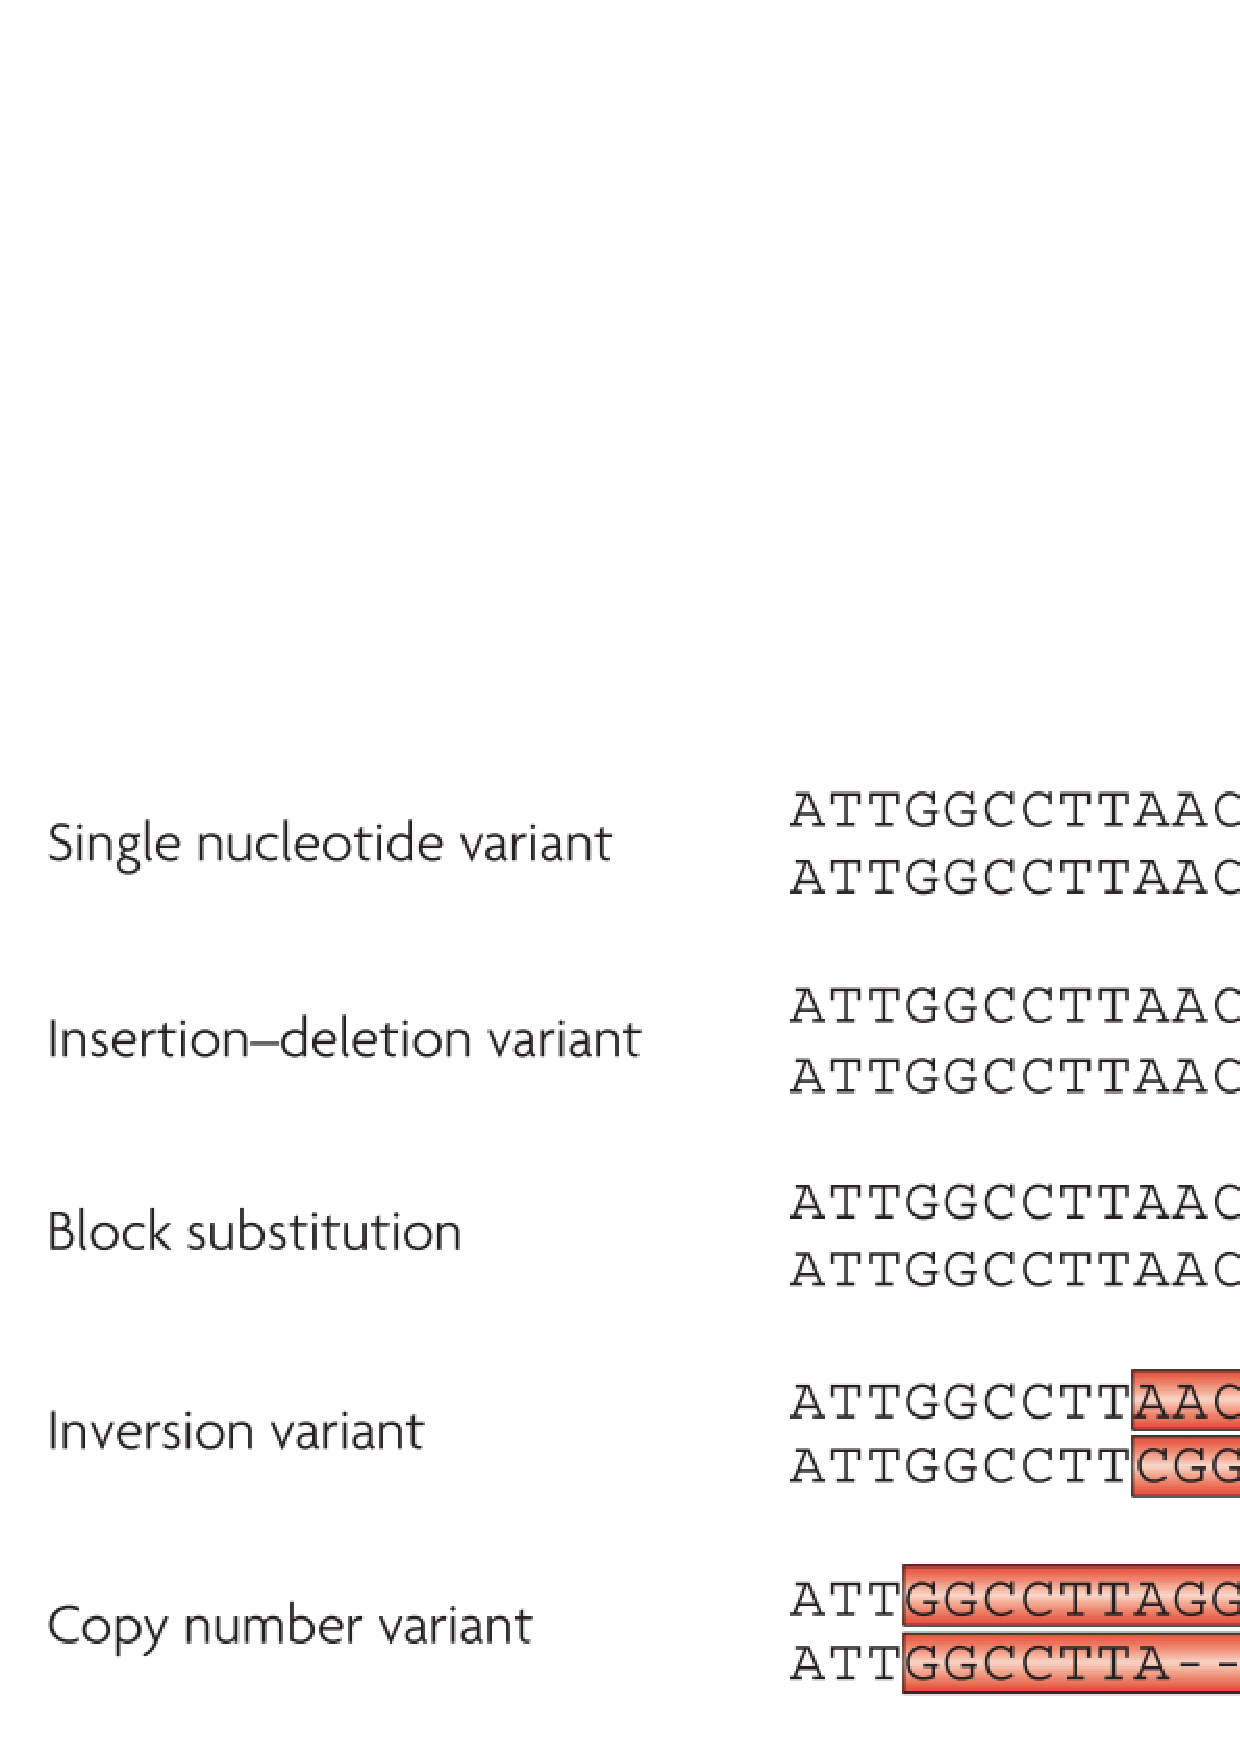
\includegraphics[width=0.3\textwidth]{/home/jennifer/Documentos/latex1/Plantilla_LaTex_UN/Kap4/variantes.png}
	\caption{Distribution of age range and gender of patients}
	\label{f:generosgeneral}
\end{figure}

\begin{figure}[h!]
	\centering
	\includegraphics[width=0.3\textwidth]{/home/jennifer/Documentos/latex1/Plantilla_LaTex_UN/Kap4/edad.png}
	\caption{Distribution of age range and gender of patients}
	\label{f:variantesgeneral}
\end{figure}

The database contains 228 patients of which 133 are female and have a total of 468,485 variants and 95 male patients with 345,239 variants obtaining a total of 803,878 variants. Figure \ref{fig:general} represents the distribution of patients by age range and Figure \ref{f:generosgeneral} represents the distribution of variants according to their type. In Figure \ref{f:generosgeneral} shows the number of variants that are synonymous and not synonymous, being the most frequent in the population, at a global level it is known that these are the most frequent types of variants\cite{Fu2013}. 

The unknown variants are the third type of variant more frequent given that there is still the problem of selecting the transcript to perform the appropriate nomenclature of the variants, so the annotator reports that they are unknown \cite{McCarthy2014}. Figure \ref{f:variantesgeneral} shows the distribution of the variants identified according to the age range, the range with the highest number of variants being patients between the ages of 0 to 10 years, given that it is the most represented population within the database.

The allelic state of the variants (zygosity) found within the database are divided into 458639 heterozygotes corresponding to 57.05\% of the total of the variants and homozygous 345239 corresponding to 42.95\%. The distribution of the zygosity of the variants can be explained from the error that can be generated in the identification of the variants given that during the call of variants it is possible that a homozygous variant is classified as heterozygous, if during the sequencing process it is identified wrongly nucleotides \cite{Babraham2016,Pirooznia2014}.

\subsection*{Textual analysis of clinical information.}
The results obtained for the frequency of words were breast, cancer, syndrome, suspicion and years. In figure \ref{fig:sin} shows the first 30 most frequent words and the word cloud of all the documents.

\begin{figure}[h!]
	\centering
	\includegraphics[width=0.3\textwidth]{/home/jennifer/Documentos/latex1/Plantilla_LaTex_UN/Kap4/sin_stop}
	\caption{Wordcloud in Spanish}
	\label{fig:sin}
\end{figure}

The frequency of words shows us the main characteristics of the clinical information, the words cancer and breast are the main phenotypes, the word syndrome is also found that can be associated with different diseases and the word suspicion refers to ambiguous diagnoses that patients may have, One of the contributions of sequencing is that based on the phenotype can help a diagnosis, between different symptoms and syndromes that can be applied to rare and complex diseases \cite{Tetreault2015a}. 

\subsubsection*{Clusters of clinical characteristics.}

\paragraph*{Data transformation}
Calculation of the tf-idf matrix, is done from inverted frequency with the equation:
$${idf}_i = \log_2 \frac{|D|}{|\{d \mid t_i \in d\}|}$$
being $|D|$ what denotes the total number of documents and where $|\{d\mid t_i \in d\}|$ in which $t_1$  appears, the matrix of tf-idf is calculated from the multiplication of the frequency of terms and the inverted frequency $\mathit{tf}_{i,j} \cdot \mathit{idf}_i$ \cite{Buckley1988}.

\begin{figure}[h!] 
	\centering
	\includegraphics[width=0.3\textwidth]{/home/jennifer/Documentos/latex1/Plantilla_LaTex_UN/Kap4/tfidf.pdf}
	\caption{TF-IDF} 
	\label{fig:IDFTF}
\end{figure}

Figure \ref{fig:IDFTF} represents the IDF-TF matrix of the words found within the database.

\subsubsection*{Clustering model validation}

Inertia was computed and  the graph of the quadratic error vs the number of clusters was made.Where cluster 5 and 6 can be selected as the optimum of $K$ .For the definition of the optimal number of $K$, we also calculate the Silhouette coefficient, which is an evaluation of the clusters. Silhouette coefficient was \textit{0.534}. 

For 5 clusters obtained, the validation measures that are inside the library scikit-learn were: For homogeneity 0.296, for integrity 1.0, for V-measure 0.457 and the Rand-Index was 0. The perfect homogeneity would be with a value of 1.0, in the present clusters they present a low homogeneity, but an integrity of 1.0 which means that the labels are perfectly complete, this is reflected in the V-measure which is 0.457 where we have clusters with low homogeneity but high integrity. Rand-Index a value of 0.0 was obtained that shows that the classes are separated into different clusters \cite{scikit-learn}.

\subsection*{Association of clusters with variants.}

Results of applying association rules to the variants along with their clusters were:

\subsubsection*{Cluster 1}

\begin{figure}[h!] 
	\centering
	\includegraphics[width=0.3\textwidth]{/home/jennifer/Documentos/latex1/Plantilla_LaTex_UN/Kap4/cluster1}
	\caption{Wordcloud cluster 1} 
	\label{f:nube1}
\end{figure}

\begin{figure}[h!] 
	\centering
	\includegraphics[width=0.3\textwidth]{/home/jennifer/Documentos/latex1/Plantilla_LaTex_UN/Kap4/edadc1}
	\caption{Cluster 1} 
	\label{fig:cluster1}
\end{figure}


\begin{figure}[h!]
	\centering
	\includegraphics[width=0.4\textwidth]{/home/jennifer/Documentos/latex1/Plantilla_LaTex_UN/Kap4/reglas1_1}
	\caption{Cluster 1 association rules with synonymous variants.} \label{fig:reglas1}
\end{figure}

The figure 	\ref{f:nube1} represents the cluster 1 with the frequency of words that were grouped for this cluster and frequency of words is shown, being breast, syndrome and cancer are the most frequent words, along with ovarian, familial suspicion and epilepsy. Figure \ref {fig:cluster1} represents the distribution of patients by age and gender within the group by age range over a 10-year interval. The first 10 rules obtained are represented by the figure \ref{fig:reglas1} that shows the association of variants with clinical information of cluster 1. The results are without removing the synonymous variants. For the present cluster there are two types of variants distributed by the male gender with nonsynonymous variants and that are patients aged between 10 and 20 years, the allelic state of the variants is homozygous, for this group a high difference is observed in the rules both genders, where female patients have synonymous variants with heterozygous status.

\subsubsection*{Cluster 2}

\begin{figure}[h!] 
	\centering
	\includegraphics[width=0.3\textwidth]{/home/jennifer/Documentos/latex1/Plantilla_LaTex_UN/Kap4/cluster2}
	\caption{Wordcloud cluster 2} 
	\label{f:nube2}
\end{figure}

\begin{figure}[h!] 
	\centering
	\includegraphics[width=0.3\textwidth]{/home/jennifer/Documentos/latex1/Plantilla_LaTex_UN/Kap4/edadc2}
	\caption{Cluster 2} 
	\label{fig:cluster2}
\end{figure}

\begin{figure}[h!]
	\centering
	\includegraphics[width=0.4\textwidth]{/home/jennifer/Documentos/latex1/Plantilla_LaTex_UN/Kap4/reglas2_1}
	\caption{Cluster 2 association rules with synonymous variants.} \label{fig:reglas2}
\end{figure}

In the figure \ref{f:nube2} is observed that like cluster 1 the most frequent words are cancer, breast and syndrome, but words like thyroid and sister antecedents appear, according to the figure \ref{fig:cluster2} is observed that age ranges between 20 and 30 years, and over 40 there are no male patients, this being a cluster represented mainly by female patients.

The figure \ref{fig: reglas2_1}, shows us only an association of variants to the female gender, which corresponds to the low representation of male patients.The distribution of the homozygous allelic state occurs more frequently with patients of the age of 30 and 40 years, and they are variants of non-synonymous type, although the age range is not the most representative of the cluster, it is the one with the highest frequency of variants.


Thus we observe that this expected value is finite for all $v>0$ (also see \cite{koon,khar,zvai,xjon,marg}).
%\nocite{oreg,schn,pond,smith,marg,hunn,advi,koha,mouse}

%%%%%%%%%%%%%%%%%%%%%%%%%%%%%%%%%%%%%%%%%%%%%%
%%                                          %%
%% Backmatter begins here                   %%
%%                                          %%
%%%%%%%%%%%%%%%%%%%%%%%%%%%%%%%%%%%%%%%%%%%%%%

\begin{backmatter}

\section*{Competing interests}
  The authors declare that they have no competing interests.

\section*{Author's contributions}
    Text for this section \ldots

\section*{Acknowledgements}
  Text for this section \ldots
%%%%%%%%%%%%%%%%%%%%%%%%%%%%%%%%%%%%%%%%%%%%%%%%%%%%%%%%%%%%%
%%                  The Bibliography                       %%
%%                                                         %%
%%  Bmc_mathpys.bst  will be used to                       %%
%%  create a .BBL file for submission.                     %%
%%  After submission of the .TEX file,                     %%
%%  you will be prompted to submit your .BBL file.         %%
%%                                                         %%
%%                                                         %%
%%  Note that the displayed Bibliography will not          %%
%%  necessarily be rendered by Latex exactly as specified  %%
%%  in the online Instructions for Authors.                %%
%%                                                         %%
%%%%%%%%%%%%%%%%%%%%%%%%%%%%%%%%%%%%%%%%%%%%%%%%%%%%%%%%%%%%%

% if your bibliography is in bibtex format, use those commands:
\bibliographystyle{bmc-mathphys} % Style BST file (bmc-mathphys, vancouver, spbasic).
\bibliography{library}      % Bibliography file (usually '*.bib' )
% for author-year bibliography (bmc-mathphys or spbasic)
% a) write to bib file (bmc-mathphys only)
% @settings{label, options="nameyear"}
% b) uncomment next line
%\nocite{label}

% or include bibliography directly:
% \begin{thebibliography}
% \bibitem{b1}
% \end{thebibliography}

%%%%%%%%%%%%%%%%%%%%%%%%%%%%%%%%%%%
%%                               %%
%% Figures                       %%
%%                               %%
%% NB: this is for captions and  %%
%% Titles. All graphics must be  %%
%% submitted separately and NOT  %%
%% included in the Tex document  %%
%%                               %%
%%%%%%%%%%%%%%%%%%%%%%%%%%%%%%%%%%%

%%
%% Do not use \listoffigures as most will included as separate files

\section*{Figures}
  \begin{figure}[h!]
  \caption{\csentence{Sample figure title.}
      A short description of the figure content
      should go here.}
      \end{figure}

\begin{figure}[h!]
  \caption{\csentence{Sample figure title.}
      Figure legend text.}
      \end{figure}

%%%%%%%%%%%%%%%%%%%%%%%%%%%%%%%%%%%
%%                               %%
%% Tables                        %%
%%                               %%
%%%%%%%%%%%%%%%%%%%%%%%%%%%%%%%%%%%

%% Use of \listoftables is discouraged.
%%
\section*{Tables}
\begin{table}[h!]
\caption{Sample table title. This is where the description of the table should go.}
      \begin{tabular}{cccc}
        \hline
           & B1  &B2   & B3\\ \hline
        A1 & 0.1 & 0.2 & 0.3\\
        A2 & ... & ..  & .\\
        A3 & ..  & .   & .\\ \hline
      \end{tabular}
\end{table}

%%%%%%%%%%%%%%%%%%%%%%%%%%%%%%%%%%%
%%                               %%
%% Additional Files              %%
%%                               %%
%%%%%%%%%%%%%%%%%%%%%%%%%%%%%%%%%%%

\section*{Additional Files}
  \subsection*{Additional file 1 --- Sample additional file title}
    Additional file descriptions text (including details of how to
    view the file, if it is in a non-standard format or the file extension).  This might
    refer to a multi-page table or a figure.

  \subsection*{Additional file 2 --- Sample additional file title}
    Additional file descriptions text.


\end{backmatter}
\end{document}
